\documentclass{article}

\usepackage{amsthm}
\usepackage{amsfonts}
\usepackage{amsmath}
\usepackage{amssymb}
\usepackage{enumitem}
\usepackage{fullpage}
\usepackage[usenames]{color}
\usepackage{hyperref}
  \hypersetup{
    colorlinks = true,
    urlcolor = blue,       % color of external links using \href
    linkcolor= blue,       % color of internal links 
    citecolor= blue,       % color of links to bibliography
    filecolor= blue,        % color of file links
    }
    
\usepackage{listings}
\usepackage{qtree}
\usepackage{tikz-qtree}

\definecolor{dkgreen}{rgb}{0,0.6,0}
\definecolor{gray}{rgb}{0.5,0.5,0.5}
\definecolor{mauve}{rgb}{0.58,0,0.82}

\lstset{frame=tb,
  language=haskell,
  aboveskip=3mm,
  belowskip=3mm,
  showstringspaces=false,
  columns=flexible,
  basicstyle={\small\ttfamily},
  numbers=none,
  numberstyle=\tiny\color{gray},
  keywordstyle=\color{blue},
  commentstyle=\color{dkgreen},
  stringstyle=\color{mauve},
  breaklines=true,
  breakatwhitespace=true,
  tabsize=3
}

\theoremstyle{theorem} 
   \newtheorem{theorem}{Theorem}[section]
   \newtheorem{corollary}[theorem]{Corollary}
   \newtheorem{lemma}[theorem]{Lemma}
   \newtheorem{proposition}[theorem]{Proposition}
\theoremstyle{definition}
   \newtheorem{definition}[theorem]{Definition}
   \newtheorem{example}[theorem]{Example}
\theoremstyle{remark}    
  \newtheorem{remark}[theorem]{Remark}


\title{CPSC-354 Report}
\author{Eleas Vrahnos  \\ Chapman University}

\date{\today}

\begin{document}

\maketitle

\begin{abstract}
To be written at a later date. 
\end{abstract}

\tableofcontents

\section{Introduction}\label{intro}

This report is written by Eleas Vrahnos. It details all assignments and progress made in the Programming Languages course at Chapman University. It includes weekly homework assigments, programming assignments, and a final project that demonstrate understanding and application in various class topics.

\section{Homework}\label{homework}

This section will contain my solutions to the weekly homework assignments. 

\subsection{Week 1}

The following is a Python implementation of the Euclidean algorithm:

\begin{lstlisting}[language=Python]
def gcd(a,b):
    while a != b:
        if a > b:
            a = a-b
        else:
            b = b-a
    return a
\end{lstlisting}

\newpage % Temporary page break

\noindent We can test this code by going through the function with a sample input \texttt{gcd(9, 33)}, step by step.

\begin{enumerate}[noitemsep]
  \item \texttt{gcd(9, 33)}
  \begin{itemize}
      \item The function is called, assigning 9 to variable \texttt{a} and 33 to variable \texttt{b}.
  \end{itemize} 
  \item \texttt{while a != b:}
  \begin{itemize}
      \item The while loop condition returns True, so the loop starts.
  \end{itemize}
  \item \texttt{else:}
  \begin{itemize}
      \item \texttt{a > b} (9 $>$ 33) returns False, so the else block executes.
  \end{itemize}
  \item \texttt{b = b-a}
  \begin{itemize}
      \item \texttt{b} is now assigned to $33 - 9$, which is $24$.
  \end{itemize}
  \item \texttt{while a != b:}
  \begin{itemize}
      \item The while loop condition returns True, so the loop starts.
  \end{itemize}
  \item \texttt{else:}
  \begin{itemize}
      \item \texttt{a > b} (9 $>$ 24) returns False, so the else block executes.
  \end{itemize}
  \item \texttt{b = b-a}
  \begin{itemize}
      \item \texttt{b} is now assigned to $24 - 9$, which is $15$.
  \end{itemize}
  \item \texttt{while a != b:}
  \begin{itemize}
      \item The while loop condition returns True, so the loop starts.
  \end{itemize}
  \item \texttt{else:}
  \begin{itemize}
      \item \texttt{a > b} (9 $>$ 15) returns False, so the else block executes.
  \end{itemize}
  \item \texttt{b = b-a}
  \begin{itemize}
      \item \texttt{b} is now assigned to $15 - 9$, which is $6$.
  \end{itemize}
  \item \texttt{while a != b:}
  \begin{itemize}
      \item The while loop condition returns True, so the loop starts.
  \end{itemize}
  \item \texttt{if a > b:}
  \begin{itemize}
      \item \texttt{a > b} (9 $>$ 6) returns True, so the first block executes.
  \end{itemize}
  \item \texttt{a = a-b}
  \begin{itemize}
      \item \texttt{a} is now assigned to $9 - 6$, which is $3$.
  \end{itemize}
  \item \texttt{while a != b:}
  \begin{itemize}
      \item The while loop condition returns True, so the loop starts.
  \end{itemize}
  \item \texttt{else:}
  \begin{itemize}
      \item \texttt{a > b} (3 $>$ 6) returns False, so the else block executes.
  \end{itemize}
  \item \texttt{b = b-a}
  \begin{itemize}
      \item \texttt{b} is now assigned to $6 - 3$, which is $3$.
  \end{itemize}
  \item \texttt{while a != b:}
  \begin{itemize}
      \item The while loop condition returns False (\texttt{3 == 3}), so the loop ends.
  \end{itemize}
  \item \texttt{return a}
  \begin{itemize}
      \item \texttt{a} is returned from the function, giving the correct greatest common divisor of \textbf{3}.
  \end{itemize}
\end{enumerate}
\subsection{Week 2}


The following are implementations of various functions in Haskell. \newline

% select_evens function
\noindent \texttt{select\_evens}, lists the even-indexed elements of a given list:
\begin{lstlisting}[language=Haskell]
-- Implementation
select_evens [] = [] -- in the case of a list with even number elements
select_evens (x:[]) = [] -- in the case of a list with odd number elements
select_evens (x:y:xs) = y : select_evens (xs)

-- Execution Sequence with example ["a","b","c","d","e"]
select_evens ["a","b","c","d","e"] =
    "b" : (select_evens["c","d","e"]) = 
    "b" : ("d" : (select_evens["e"])) =
    "b" : ("d" : ([])) = 
    ["b","d"]
\end{lstlisting} 

% select_odds function
\noindent \texttt{select\_odds}, lists the odd-indexed elements of a given list:
\begin{lstlisting}[language=Haskell]
-- Implementation
select_odds [] = [] -- in the case of a list with even number elements
select_odds (x:[]) = [x] -- in the case of a list with odd number elements
select_odds (x:y:xs) = x : select_odds (xs)

-- Execution Sequence with example ["a","b","c","d","e"]
select_odds ["a","b","c","d","e"] =
    "a" : (select_odds["c","d","e"]) = 
    "a" : ("c" : (select_odds["e"])) =
    "a" : ("c" : ("e")) = 
    ["a","c","e"]
\end{lstlisting}

% member function
\noindent \texttt{member}, determines whether an element is part of a given list:
\begin{lstlisting}[language=Haskell]
-- Implementation
member a [] = False
member a (x:xs)
    | a==x = True
    | otherwise = member a (xs)

-- Execution Sequence with example 2 [5,2,6]
member 2 [5,2,6] =
    member 2 [2,6] = 
    True
\end{lstlisting}

\newpage % Temporary page break

% append function
\noindent \texttt{append}, appends a list to another list:
\begin{lstlisting}[language=Haskell]
-- Implementation
append [] ys = ys
append (x:xs) ys = x : append xs ys

-- Execution Sequence with example [1,2] [3,4,5]
append [1,2] [3,4,5] =
    1 : (append [2] [3,4,5]) = 
    1 : (2 : (append [] [3,4,5])) =
    1 : (2 : ([3,4,5])) =
    [1,2,3,4,5]
\end{lstlisting}

% revert function
\noindent \texttt{revert}, reverses a list:
\begin{lstlisting}[language=Haskell]
-- Implementation
revert [] = []
revert (x:xs) = append (revert(xs)) [x]

-- Execution Sequence with example [1,2,3]
revert [1,2,3] =
    append (revert [2,3]) [1] =
    append (append (revert [3]) [2]) [1] =
    append (append (append (revert []) [3]) [2]) [1] =
    append (append (append [] [3]) [2]) [1] =
    append (append [3] [2]) [1] = 
    append (3 : (append [] [2])) [1] =
    append (3 : [2]) [1] =
    append [3,2] [1] =
    3 : (append [2] [1]) =
    3 : (2 : (append [] [1]) =
    3 : (2 : [1]) =
    [3,2,1]
\end{lstlisting}

% less_equal function
\noindent \texttt{less\_equal}, checks if the element in a list is less than or equal to the same-indexed element in another list:
\begin{lstlisting}[language=Haskell]
-- Implementation
less_equal [] [] = True
less_equal (x:xs) (y:ys)
    | x > y = False
    | otherwise = less_equal (xs) (ys)

-- Execution Sequence with example [1,2,3] [2,3,2]
less_equal [1,2,3] [2,3,2] =
    less_equal [2,3] [3,2] = 
    less_equal [3] [2] = 
    False
\end{lstlisting}

\newpage % Temporary page break
\subsection{Week 3}

The following investigates the Tower of Hanoi problem. Here is a given Haskell implementation describing moves in the game, as well as the execution sequence for the test input \texttt{hanoi 5 0 2}.
\begin{lstlisting}[language=Haskell]
-- Implementation
hanoi 1 x y = move x y

hanoi (n+1) x y = 
    hanoi n x (other x y) 
    move x y 
    hanoi n (other x y) y

-- Execution Sequence
hanoi 5 0 2
    hanoi 4 0 1
        hanoi 3 0 2
            hanoi 2 0 1
                hanoi 1 0 2 = move 0 2
                move 0 1
                hanoi 1 2 1 = move 2 1
            move 0 2
            hanoi 2 1 2
                hanoi 1 1 0 = move 1 0
                move 1 2
                hanoi 1 0 2 = move 0 2
        move 0 1
        hanoi 3 2 1
            hanoi 2 2 0
                hanoi 1 2 1 = move 2 1
                move 2 0
                hanoi 1 1 0 = move 1 0
            move 2 1
            hanoi 2 0 1
                hanoi 1 0 2 = move 0 2
                move 0 1
                hanoi 1 2 1 = move 2 1
    move 0 2
    hanoi 4 1 2
        hanoi 3 1 0
            hanoi 2 1 2
                hanoi 1 1 0 = move 1 0
                move 1 2
                hanoi 1 0 2 = move 0 2
            move 1 0
            hanoi 2 2 0
                hanoi 1 2 1 = move 2 1
                move 2 0
                hanoi 1 1 0 = move 1 0
        move 1 2
        hanoi 3 0 2
            hanoi 2 0 1
                hanoi 1 0 2 = move 0 2
                move 0 1
                hanoi 1 2 1 = move 2 1
            move 0 2
            hanoi 2 1 2
                hanoi 1 1 0 = move 1 0
                move 1 2
                hanoi 1 0 2 = move 0 2
\end{lstlisting} 
From this execution, the moves for a 5-ring Tower of Hanoi game can be seen as follows:
\begin{lstlisting}
0->2, 0->1, 2->1, 0->2, 1->0, 1->2, 0->2, 0->1, 2->1, 2->0, 1->0, 2->1, 0->2, 0->1, 2->1, 0->2, 1->0, 1->2, 0->2, 1->0, 2->1, 2->0, 1->0, 1->2, 0->2, 0->1, 2->1, 0->2, 1->0, 1->2, 0->2
\end{lstlisting}

\noindent \textbf{Analysis:} From this computation, the word \texttt{hanoi} appears exactly 31 times in the execution. Based on executions of the game with a different number of starting rings, the formula $2^n - 1$ can be derived to determine how many times \texttt{hanoi} will appear, with \texttt{n} being the number of disks in the game.
\subsection{Week 4}
The following compares concrete and abstract syntax trees of various mathematical expressions.

The expression $2+1$:\newline

\hfil
\begin{tikzpicture}
\begin{scope}
\Tree[.Exp [.Exp [.Exp1 [.Exp2 $3$ ]]]
           [.+ ]
           [.Exp1 [.Exp2 $1$ ]]]
\end{scope}
\begin{scope}[xshift=5cm]
\Tree[.Plus [.2 ]
            [.1 ]]
\end{scope}
\end{tikzpicture}
\hfil

The expression $1+2*3$:\newline

\hfil
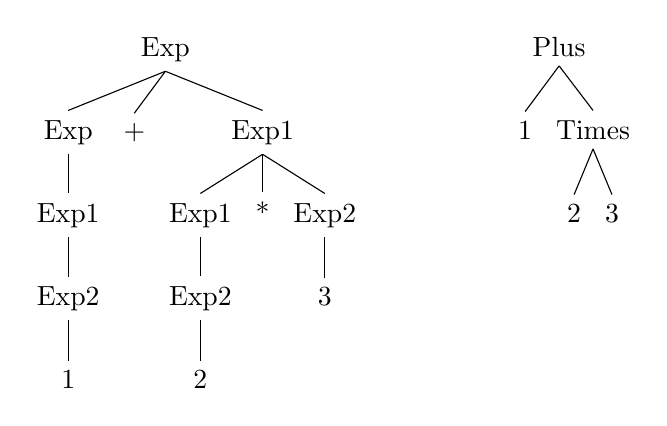
\begin{tikzpicture}
\begin{scope}
\Tree[.Exp [.Exp [.Exp1 [.Exp2 $1$ ]]]
           [.+ ]
           [.Exp1 [.Exp1 [.Exp2 $2$ ]]
                  [.* ]
                  [.Exp2 $3$ ]]]
\end{scope}

\begin{scope}[xshift=5cm]
\Tree[.Plus [.1 ]
            [.Times [.2 ]
                    [.3 ]]]
\end{scope}
\end{tikzpicture}
\hfil

\newpage
The expression $1+(2*3)$:\newline

\hfil
\begin{tikzpicture}
\begin{scope}
\Tree[.Exp [.Exp [.Exp1 [.Exp2 $1$ ]]]
           [.+ ]
           [.Exp1 [.Exp2 [.( ]
                         [.Exp [.Exp1 [.Exp1 [.Exp2 $1$ ]]
                                      [.* ]
                                      [.Exp2 $3$ ]]]
                         [.) ]]]]
                         
\end{scope}

\begin{scope}[xshift=5cm]
\Tree[.Plus [.1 ]
            [.Times [.2 ]
                    [.3 ]]]
\end{scope}
\end{tikzpicture}
\hfil    

The expression $(1+2)*3$:\newline

\hfil
\begin{tikzpicture}
\begin{scope}
\Tree[.Exp [.Exp1 [.Exp1 [.Exp2 [.( ]
                                [.Exp [.Exp [.Exp1 [.Exp2 $1$ ]]]
                                      [.+ ]
                                      [.Exp1 [.Exp2 $2$ ]]]
                                [.) ]]]
           [.* ]
           [.Exp2 $3$ ]]]
                         
\end{scope}

\begin{scope}[xshift=5cm]
\Tree[.Times [.Plus [.1 ]
                    [.2 ]]
             [.3 ]]
\end{scope}
\end{tikzpicture}
\hfil

\newpage
The expression $1+2*3+4*5+6$:\newline

\hfil
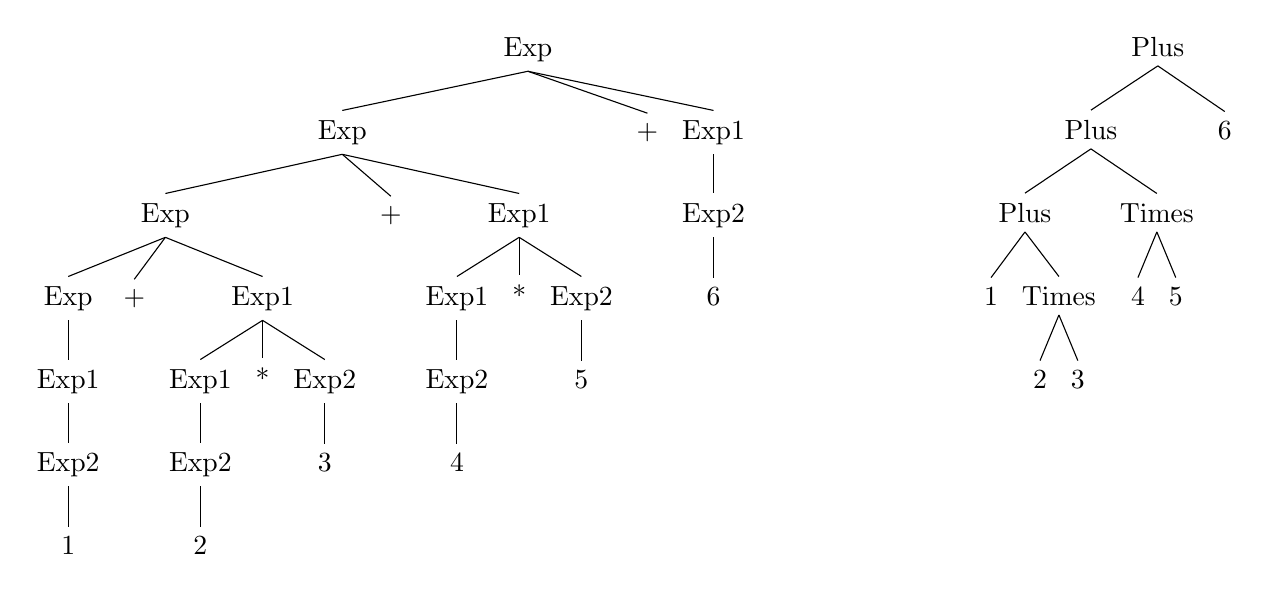
\begin{tikzpicture}
\begin{scope}
\Tree[.Exp [.Exp [.Exp [.Exp [.Exp1 [.Exp2 $1$ ]]]
                       [.+ ]
                       [.Exp1 [.Exp1 [.Exp2 $2$ ]]
                              [.* ]
                              [.Exp2 $3$ ]]]
                 [.+ ]
                 [.Exp1 [.Exp1 [.Exp2 $4$ ]]
                        [.* ]
                        [.Exp2 $5$ ]]]
           [.+ ]
           [.Exp1 [.Exp2 $6$ ]]]
                

                         
\end{scope}

\begin{scope}[xshift=8cm]
\Tree[.Plus [.Plus [.Plus [.1 ]
                          [.Times [.2 ]
                                  [.3 ]]]
                   [.Times [.4 ]
                           [.5 ]]]
            [.6 ]]

                   
\end{scope}
\end{tikzpicture}
\hfil

\noindent \textbf{Analysis of the abstract syntax tree of $1+2+3$}:
The abstract syntax tree of $1+2+3$ would match the tree of $(1+2)+3$. This is because the first breakdown of $+$ separates it to \texttt{Exp} and \texttt{Exp1}, and \texttt{Exp1} cannot reduce down to another sum. Therefore, the right side of the tree must become an integer, while the left side reduces down to a sum. The resulting tree would be as follows, which matches $(1+2)+3$ and not $1+(2+3)$.

\hfil
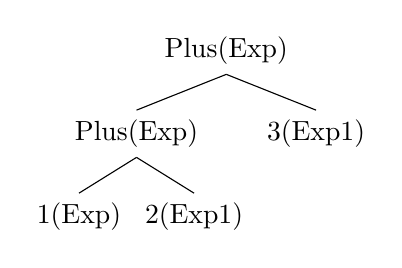
\begin{tikzpicture}
\Tree[.Plus(Exp) [.Plus(Exp) [.1(Exp) ]
                             [.2(Exp1) ]]
                 [.3(Exp1) ]]
\end{tikzpicture}
\hfil

\subsection{Week 5}
After generating a working parser demonstrating lambda calculus, linearized abstract syntax trees and 2-dimensional notation abstract syntax trees can be generated for the below expressions.
\begin{lstlisting}[language=Haskell]
-- x
x 
Prog (EVar (Id "x"))
\end{lstlisting}

\hfil
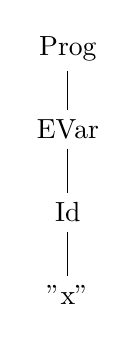
\begin{tikzpicture}
\Tree[.Prog [.EVar [.Id [."x" ]]]]
\end{tikzpicture}
\hfil

\newpage
\begin{lstlisting}[language=Haskell]
-- x x
x x
Prog (EApp (EVar (Id "x")) (EVar (Id "x")))
\end{lstlisting}

\hfil
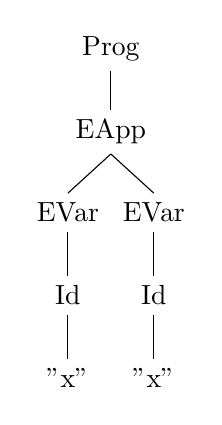
\begin{tikzpicture}
\Tree[.Prog [.EApp [.EVar [.Id [."x" ]]]
                   [.EVar [.Id [."x" ]]]]]
\end{tikzpicture}
\hfil

\begin{lstlisting}[language=Haskell]
-- x y
x y
Prog (EApp (EVar (Id "x")) (EVar (Id "y")))
\end{lstlisting}

\hfil
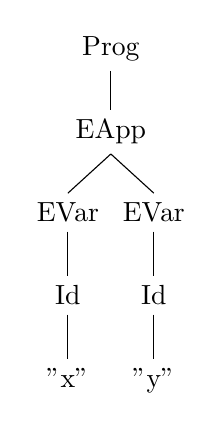
\begin{tikzpicture}
\Tree[.Prog [.EApp [.EVar [.Id [."x" ]]]
                   [.EVar [.Id [."y" ]]]]]
\end{tikzpicture}
\hfil

\begin{lstlisting}[language=Haskell]
-- x y z
x y z
Prog (EApp (EApp (EVar (Id "x")) (EVar (Id "y"))) (EVar (Id "z")))
\end{lstlisting}

\hfil
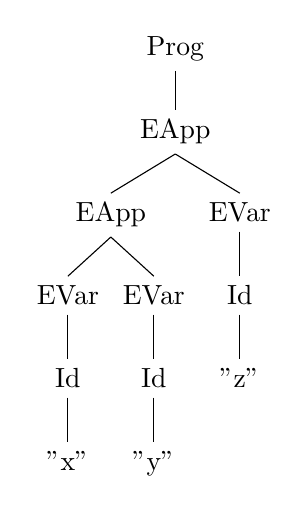
\begin{tikzpicture}
\Tree[.Prog [.EApp [.EApp [.EVar [.Id [."x" ]]]
                          [.EVar [.Id [."y" ]]]]
                   [.EVar [.Id [."z" ]]]]]
\end{tikzpicture}
\hfil

\begin{lstlisting}[language=Haskell]
-- \ x.x
\ x . x
Prog (EAbs (Id "x") (EVar (Id "x")))
\end{lstlisting}

\hfil
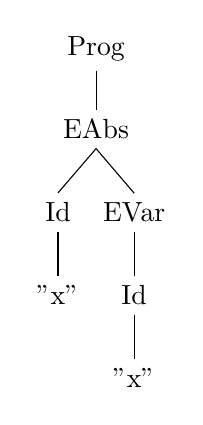
\begin{tikzpicture}
\Tree[.Prog [.EAbs [.Id [."x" ]]
                   [.EVar [.Id [."x" ]]]]]
\end{tikzpicture}
\hfil

\begin{lstlisting}[language=Haskell]
-- \ x.x x
\ x . x x
Prog (EAbs (Id "x") (EApp (EVar (Id "x")) (EVar (Id "x"))))
\end{lstlisting}

\hfil
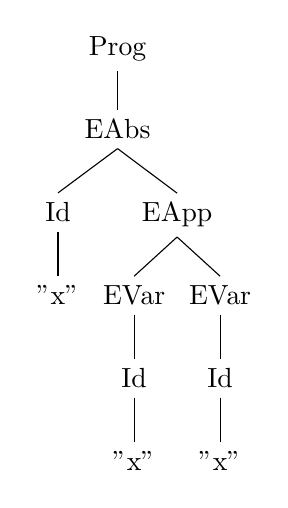
\begin{tikzpicture}
\Tree[.Prog [.EAbs [.Id [."x" ]]
                   [.EApp [.EVar [.Id [."x" ]]]
                          [.EVar [.Id [."x" ]]]]]]
\end{tikzpicture}
\hfil

\newpage
\begin{lstlisting}[language=Haskell]
-- (\ x . (\ y . x y)) (\ x.x) z
\ x . \ y . x y (\ x . x)z
Prog (EApp (EApp (EAbs (Id "x") (EAbs (Id "y") (EApp (EVar (Id "x")) (EVar (Id "y"))))) (EAbs (Id "x") (EVar (Id "x")))) (EVar (Id "z")))
\end{lstlisting}

\hfil
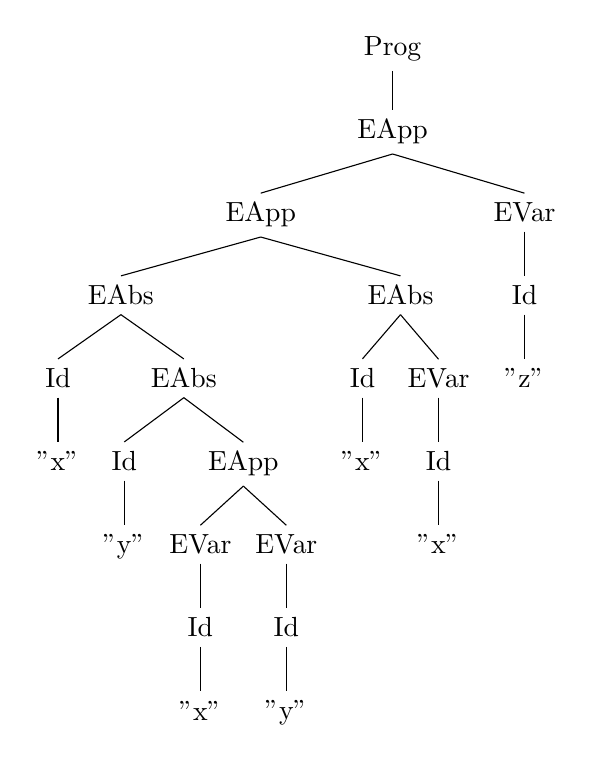
\begin{tikzpicture}
\Tree[.Prog [.EApp [.EApp [.EAbs [.Id [."x" ]]
                                 [.EAbs [.Id [."y" ]]
                                        [.EApp [.EVar [.Id [."x" ]]]
                                               [.EVar [.Id [."y" ]]]]]]
                          [.EAbs [.Id [."x" ]]
                                 [.EVar [.Id [."x" ]]]]]
                   [.EVar [.Id [."z" ]]]]]
\end{tikzpicture}
\hfil

\newpage
\begin{lstlisting}[language=Haskell]
-- (\ x . \ y . x y z) a b c
\ x . \ y . x y z a b c
Prog (EApp (EApp (EApp (EAbs (Id "x") (EAbs (Id "y") (EApp (EApp (EVar (Id "x")) (EVar (Id "y"))) (EVar (Id "z"))))) (EVar (Id "a"))) (EVar (Id "b"))) (EVar (Id "c")))
\end{lstlisting}

\hfil
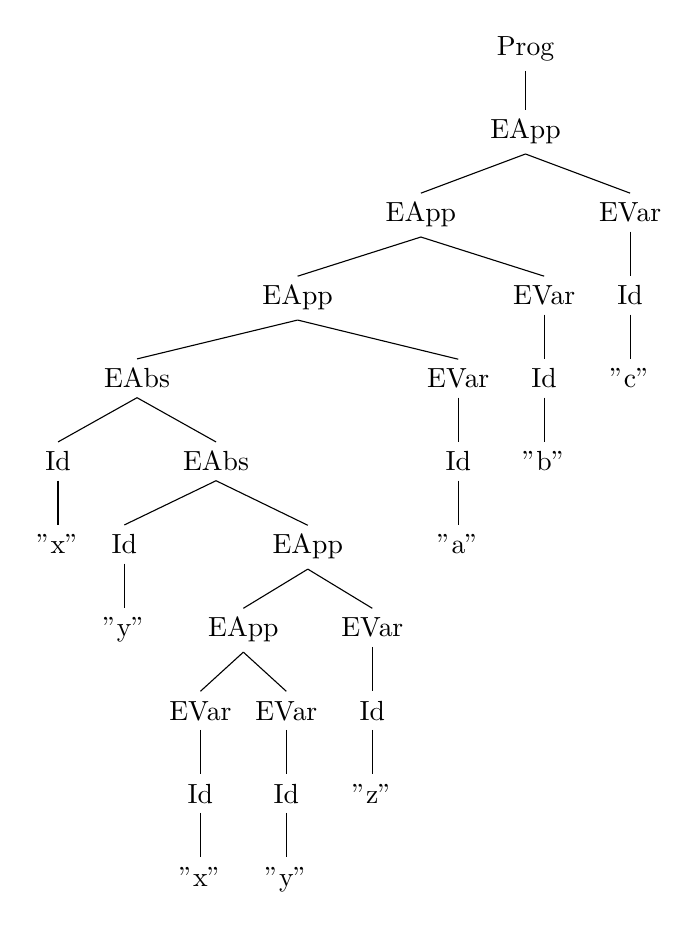
\begin{tikzpicture}
\Tree[.Prog [.EApp [.EApp [.EApp [.EAbs [.Id [."x" ]]
                                        [.EAbs [.Id [."y" ]]
                                               [.EApp [.EApp [.EVar [.Id [."x" ]]]
                                                             [.EVar [.Id [."y" ]]]]
                                                      [.EVar [.Id [."z" ]]]]]]
                                 [.EVar [.Id [."a" ]]]]
                          [.EVar [.Id [."b" ]]]]
                   [.EVar [.Id [."c" ]]]]]
\end{tikzpicture}
\hfil

\noindent The following will show the reduction of several lambda calculus expressions.
\begin{lstlisting}[language=Haskell]
(\x.x) a =
    a
\end{lstlisting}
\begin{lstlisting}[language=Haskell]
\x.x a =
    \x.x a
\end{lstlisting}
\begin{lstlisting}[language=Haskell]
(\x.\y.x) a b =
    (\y.a) b =
    a
\end{lstlisting}
\begin{lstlisting}[language=Haskell]
(\x.\y.y) a b =
    (\y.y) b =
    b
\end{lstlisting}
\newpage
\begin{lstlisting}[language=Haskell]
(\x.\y.x) a b c =
    (\y.a) b c =
    a c
\end{lstlisting}
\begin{lstlisting}[language=Haskell]
(\x.\y.y) a b c =
    (\y.a) b c =
    b c
\end{lstlisting}
\begin{lstlisting}[language=Haskell]
(\x.\y.x) a (b c) =
    (\y.a) (b c) =
    a
\end{lstlisting}
\begin{lstlisting}[language=Haskell]
(\x.\y.y) a (b c) =
    (\y.y) (b c) =
    b c
\end{lstlisting}
\begin{lstlisting}[language=Haskell]
(\x.\y.x) (a b) c =
    (\y.(a b)) c =
    a b
\end{lstlisting}
\begin{lstlisting}[language=Haskell]
(\x.\y.y) (a b) c =
    (\y.y) c =
    c
\end{lstlisting}
\begin{lstlisting}[language=Haskell]
(\x.\y.x) (a b c) =
    \y.(a b c)
\end{lstlisting}
\begin{lstlisting}[language=Haskell]
(\x.\y.y) (a b c) =
    \y.y
\end{lstlisting}
\begin{lstlisting}[language=Haskell]
evalCBN (\x.x)((\y.y)a) =
    evalCBN (EApp (EAbs (Id "x") (EVar (Id "x"))) (EApp (EAbs (Id "y") (EVar (Id "y"))) (EVar (Id "a")))) =
    evalCBN (subst (Id "x") (EApp (EAbs (Id "y") (EVar (Id "y"))) (EVar (Id "a"))) (EVar (Id "x"))) =
    evalCBN (EApp (EAbs (Id "y") (EVar (Id "y"))) (EVar (Id "a"))) =
    evalCBN (subst (Id "y") (EVar (Id "a")) (EVar (Id "y"))) =
    EVar (Id "a")
\end{lstlisting}

\section{Project}

To be written at a later date.

\section{Conclusions}\label{conclusions}

To be written at a later date.

\end{document}